% Options for packages loaded elsewhere
\PassOptionsToPackage{unicode}{hyperref}
\PassOptionsToPackage{hyphens}{url}
%
\documentclass[
  man,mask,floatsintext]{apa6}
\usepackage{amsmath,amssymb}
\usepackage{lmodern}
\usepackage{iftex}
\ifPDFTeX
  \usepackage[T1]{fontenc}
  \usepackage[utf8]{inputenc}
  \usepackage{textcomp} % provide euro and other symbols
\else % if luatex or xetex
  \usepackage{unicode-math}
  \defaultfontfeatures{Scale=MatchLowercase}
  \defaultfontfeatures[\rmfamily]{Ligatures=TeX,Scale=1}
\fi
% Use upquote if available, for straight quotes in verbatim environments
\IfFileExists{upquote.sty}{\usepackage{upquote}}{}
\IfFileExists{microtype.sty}{% use microtype if available
  \usepackage[]{microtype}
  \UseMicrotypeSet[protrusion]{basicmath} % disable protrusion for tt fonts
}{}
\makeatletter
\@ifundefined{KOMAClassName}{% if non-KOMA class
  \IfFileExists{parskip.sty}{%
    \usepackage{parskip}
  }{% else
    \setlength{\parindent}{0pt}
    \setlength{\parskip}{6pt plus 2pt minus 1pt}}
}{% if KOMA class
  \KOMAoptions{parskip=half}}
\makeatother
\usepackage{xcolor}
\usepackage{graphicx}
\makeatletter
\def\maxwidth{\ifdim\Gin@nat@width>\linewidth\linewidth\else\Gin@nat@width\fi}
\def\maxheight{\ifdim\Gin@nat@height>\textheight\textheight\else\Gin@nat@height\fi}
\makeatother
% Scale images if necessary, so that they will not overflow the page
% margins by default, and it is still possible to overwrite the defaults
% using explicit options in \includegraphics[width, height, ...]{}
\setkeys{Gin}{width=\maxwidth,height=\maxheight,keepaspectratio}
% Set default figure placement to htbp
\makeatletter
\def\fps@figure{htbp}
\makeatother
\setlength{\emergencystretch}{3em} % prevent overfull lines
\providecommand{\tightlist}{%
  \setlength{\itemsep}{0pt}\setlength{\parskip}{0pt}}
\setcounter{secnumdepth}{-\maxdimen} % remove section numbering
% Make \paragraph and \subparagraph free-standing
\ifx\paragraph\undefined\else
  \let\oldparagraph\paragraph
  \renewcommand{\paragraph}[1]{\oldparagraph{#1}\mbox{}}
\fi
\ifx\subparagraph\undefined\else
  \let\oldsubparagraph\subparagraph
  \renewcommand{\subparagraph}[1]{\oldsubparagraph{#1}\mbox{}}
\fi
\newlength{\cslhangindent}
\setlength{\cslhangindent}{1.5em}
\newlength{\csllabelwidth}
\setlength{\csllabelwidth}{3em}
\newlength{\cslentryspacingunit} % times entry-spacing
\setlength{\cslentryspacingunit}{\parskip}
\newenvironment{CSLReferences}[2] % #1 hanging-ident, #2 entry spacing
 {% don't indent paragraphs
  \setlength{\parindent}{0pt}
  % turn on hanging indent if param 1 is 1
  \ifodd #1
  \let\oldpar\par
  \def\par{\hangindent=\cslhangindent\oldpar}
  \fi
  % set entry spacing
  \setlength{\parskip}{#2\cslentryspacingunit}
 }%
 {}
\usepackage{calc}
\newcommand{\CSLBlock}[1]{#1\hfill\break}
\newcommand{\CSLLeftMargin}[1]{\parbox[t]{\csllabelwidth}{#1}}
\newcommand{\CSLRightInline}[1]{\parbox[t]{\linewidth - \csllabelwidth}{#1}\break}
\newcommand{\CSLIndent}[1]{\hspace{\cslhangindent}#1}
\ifLuaTeX
\usepackage[bidi=basic]{babel}
\else
\usepackage[bidi=default]{babel}
\fi
\babelprovide[main,import]{english}
% get rid of language-specific shorthands (see #6817):
\let\LanguageShortHands\languageshorthands
\def\languageshorthands#1{}
% Manuscript styling
\usepackage{upgreek}
\captionsetup{font=singlespacing,justification=justified}

% Table formatting
\usepackage{longtable}
\usepackage{lscape}
% \usepackage[counterclockwise]{rotating}   % Landscape page setup for large tables
\usepackage{multirow}		% Table styling
\usepackage{tabularx}		% Control Column width
\usepackage[flushleft]{threeparttable}	% Allows for three part tables with a specified notes section
\usepackage{threeparttablex}            % Lets threeparttable work with longtable

% Create new environments so endfloat can handle them
% \newenvironment{ltable}
%   {\begin{landscape}\centering\begin{threeparttable}}
%   {\end{threeparttable}\end{landscape}}
\newenvironment{lltable}{\begin{landscape}\centering\begin{ThreePartTable}}{\end{ThreePartTable}\end{landscape}}

% Enables adjusting longtable caption width to table width
% Solution found at http://golatex.de/longtable-mit-caption-so-breit-wie-die-tabelle-t15767.html
\makeatletter
\newcommand\LastLTentrywidth{1em}
\newlength\longtablewidth
\setlength{\longtablewidth}{1in}
\newcommand{\getlongtablewidth}{\begingroup \ifcsname LT@\roman{LT@tables}\endcsname \global\longtablewidth=0pt \renewcommand{\LT@entry}[2]{\global\advance\longtablewidth by ##2\relax\gdef\LastLTentrywidth{##2}}\@nameuse{LT@\roman{LT@tables}} \fi \endgroup}

% \setlength{\parindent}{0.5in}
% \setlength{\parskip}{0pt plus 0pt minus 0pt}

% Overwrite redefinition of paragraph and subparagraph by the default LaTeX template
% See https://github.com/crsh/papaja/issues/292
\makeatletter
\renewcommand{\paragraph}{\@startsection{paragraph}{4}{\parindent}%
  {0\baselineskip \@plus 0.2ex \@minus 0.2ex}%
  {-1em}%
  {\normalfont\normalsize\bfseries\itshape\typesectitle}}

\renewcommand{\subparagraph}[1]{\@startsection{subparagraph}{5}{1em}%
  {0\baselineskip \@plus 0.2ex \@minus 0.2ex}%
  {-\z@\relax}%
  {\normalfont\normalsize\itshape\hspace{\parindent}{#1}\textit{\addperi}}{\relax}}
\makeatother

% \usepackage{etoolbox}
\makeatletter
\patchcmd{\HyOrg@maketitle}
  {\section{\normalfont\normalsize\abstractname}}
  {\section*{\normalfont\normalsize\abstractname}}
  {}{\typeout{Failed to patch abstract.}}
\patchcmd{\HyOrg@maketitle}
  {\section{\protect\normalfont{\@title}}}
  {\section*{\protect\normalfont{\@title}}}
  {}{\typeout{Failed to patch title.}}
\makeatother

\usepackage{xpatch}
\makeatletter
\xapptocmd\appendix
  {\xapptocmd\section
    {\addcontentsline{toc}{section}{\appendixname\ifoneappendix\else~\theappendix\fi\\: #1}}
    {}{\InnerPatchFailed}%
  }
{}{\PatchFailed}
\keywords{Systematicity, Phonological development, preferential attachment, networks analysis}
\usepackage{lineno}

\linenumbers
\usepackage{csquotes}
\DeclareDelayedFloatFlavor{kableExtra}{table}
\usepackage{tipa}
\ifLuaTeX
  \usepackage{selnolig}  % disable illegal ligatures
\fi
\IfFileExists{bookmark.sty}{\usepackage{bookmark}}{\usepackage{hyperref}}
\IfFileExists{xurl.sty}{\usepackage{xurl}}{} % add URL line breaks if available
\urlstyle{same} % disable monospaced font for URLs
\hypersetup{
  pdftitle={Phonological Networks and Systematicity in Early Lexical Acquisition},
  pdflang={en-EN},
  pdfkeywords={Systematicity, Phonological development, preferential attachment, networks analysis},
  hidelinks,
  pdfcreator={LaTeX via pandoc}}

\title{Phonological Networks and Systematicity in Early Lexical Acquisition}
\author{Catherine E. Laing\textsuperscript{1}}
\date{}


\shorttitle{Systematicity in early phonological development}

\authornote{

Correspondence concerning this article should be addressed to Catherine E. Laing, Department of Language and Linguistic Science, University of York, Heslington, YO10 5DD.. E-mail: \href{mailto:catherine.laing@york.ac.uk}{\nolinkurl{catherine.laing@york.ac.uk}}

}

\affiliation{\vspace{0.5cm}\textsuperscript{1} University of York, York, UK}

\abstract{%
Infants' early words tend to be phonologically similar. This may reflect a systematic approach to early production, as they adapt newly-acquired forms to fit familiar structures in the output. This `rich-get-richer' approach to phonological acquisition, known as \emph{preferential attachment} in network science, proposes that new words cluster together with existing phonologically-similar words in the lexicon (or network). This contrasts with recent work (e.g.~Fourtassi et al., 2020) showing that the learning environment is the key predictor in learning (\emph{preferential acquisition}). This study expands on previous analyses of vocabulary norm data to analyse naturalistic data, namely phonetic transcriptions of nine infants' word productions, from word onset to age 2;6. Network growth models test whether 1) acquisition is best modelled through preferential attachment or preferential acquisition, 2) the trajectory of network growth changes over time, and 3) there are any differences in network growth of adult target forms vs.~infants' actual productions. Results show that preferential attachment predicts acquisition of new words more convincingly than preferential acquisition: newly-acquired words are phonologically similar to existing words in the network. Furthermore, systematicity is most apparent in early acquisition, and infants produce their early words more systematically than we would expect from looking at target forms alone.
}



\begin{document}
\maketitle

Decades of work on phonological development has documented the systematic nature of infants' earliest words. Studies of phonetic (McCune \& Vihman, 2001) and phonological structures (Vihman, 2016) show that many of a child's first word forms share similar properties. Infants draw on what they know: when articulatory, memory and planning capacities are simultaneously limited, a ``phonic core of remembered lexical items and articulations'' (Ferguson \& Farwell, 1975, p. 112) may help them deal with the challenge of developing an early lexicon. Vihman (2019, p. 263) describes the early lexicon as ``an emergent network of related forms'' that develops systematically, in line with the well-rehearsed segments and structures already in the infant's inventory. A networks approach to phonological development offers one way of identifying and quantifying this systematicity. In this study, I present a longitudinal analysis of nine infants' lexical development to identify systematicity in the first three years of word production. I consider the phonological characteristics of the developing lexicon using network analysis to demonstrate how early systematicity may be integral to the developing linguistic system by supporting infants to acquire the requisite capacity for flexible and automatic word production.

In early development, the combined challenges of articulation, memory and planning mean that the constraints on infants' production are high, and so they draw on a limited set of vocal outputs that represent a growing number of target words. According to Vihman (2014, 2019), word production begins with a small lexicon of phonologically-simple and accurately-produced forms, which are `selected' for their ease of production, as well as their perceptual salience. As the lexicon grows, target forms that do not necessarily fit these structures are `adapted' so that they do. Selection of and adaption to accessible phonological structures indicate the presence of systematicity within the developing lexicon. Essentially, the new target form is allocated to one of a small number of accessible or well-rehearsed motoric categories, and as these categories increase in size they become increasingly entrenched (Thelen \& Smith, 1996). In data from their bilingual (English-Spanish) daughter's early word acquisition, Deuchar and Quay (2000) show that 13 of her first 20 words are produced with a CV structure, and many are phonologically identical: she produces \emph{car}, \emph{clock}, \emph{casa} `house' and \emph{cat} as {[}ka{]}, and \emph{papa} `daddy', \emph{pájaro} `bird' and \emph{panda} as {[}pa{]}. This demonstrates a `pattern force', whereby production is driven by a small number of well-rehearsed structures. This tendency to acquire similar-sounding forms may continue throughout development: Mitchell, Tsui and Byers-Heinlein (2022) show that French-English bilingual infants are more likely to acquire translation equivalents that are similar in phonological form (cognates, e.g.~\emph{banana} and \emph{banane}) than non-cognate word pairs (e.g.~\emph{dog} and \emph{chien}) upto age 27 months. Systematicity in phonological acquisition may thus support lexical development over the first three years.

One way of interrogating systematicity in early phonological productions is through network analysis, which offers a quantitative perspective on the organization and development of the lexicon. Developmental research in this area centres around the words that children target in production to establish connectivity on phonological (e.g. Siew \& Vitevitch, 2020) and semantic (e.g. Hills, Maouene, Maouene, Sheya, \& Smith, 2009) planes. That is, how similar target words are to one another in form or meaning, and what this might mean for acquisition. However, as yet there is no work looking at the way children \emph{produce} those words; that is, whether or not children are drawing on systematicity in the output. Given the extensive background research that suggests a systematic approach to early word \emph{production}, expanding network analysis to this area is a natural next step for language development networks.

The term \emph{network} refers to a web of forms (or \emph{nodes}, in network terms) that are interconnected based on shared properties. Here these are phonological properties, but could also be semantic, or indeed non-linguistic properties such as genetic information, social connections or location (see Bell et al., 2017, for a review). Network growth models analyse changes within a system over time, and two key models\footnote{A third model - Lure of the Associates - has also been considered in some studies (Hills et al., 2009; Siew \& Vitevitch, 2020) but will not be considered here as there is no conclusive evidence for this model in the development literature.} of development have been proposed for lexical acquisition: preferential attachment (hereafter \textbf{PAT}) and preferential acquisition (hereafter \textbf{PAQ}, Hills et al., 2009; see also Steyvers \& Tenenbaum, 2005). PAT models of network growth propose a rich-get-richer scenario, whereby the most highly-connected nodes (nodes with more \emph{edges}) in the network are most likely to attract new nodes. In phonological development terms, this model implies that the lexicon will constitute clusters of similar-sounding words, and that a child is more likely to acquire new words that attach to these dense clusters: infants' production of newly-acquired words will be similar to their production of existing words in the lexicon. PAT-like growth is therefore driven by the \emph{internal} linguistic system. On the other hand, PAQ-like growth assumes that forms that connect to (i.e.~share properties with) a higher number of \emph{different} nodes in the existing network will be acquired first. PAQ models of network growth thus assume that \emph{external} factors in the learning environment influence acquisition -- that is, words that are most well-connected within the target language will be acquired earlier. In phonological terms, this would mean that early productions would constitute a more even distribution of segments and structures, resembling the statistical properties of the ambient language more closely, rather than a `pattern force' driven by dominant features of the existing lexicon.

Existing studies show mixed evidence for PAT- and PAQ-like growth\footnote{Note that these are not mutually exclusive.} in lexical development. Hills and colleagues' (2009) study of semantic networks showed evidence for PAQ, but not PAT, in associative networks of normed vocabulary acquisition data. Amatuni and Bergelson (2017) support this with an analysis of a large-scale corpus of input data combined with normed productive vocabulary data derived from WordBank (Frank, Braginsky, Yurovsky, \& Marchman, 2017). These same approaches have also been applied to phonological data: Fourtassi, Bian and Frank (2020) analyse both phonological and semantic network growth from vocabulary norms (receptive and productive) in 10 languages to find consistent evidence in support of PAQ-like growth, for both phonological and semantic networks, receptive and productive vocabularies, and across the 10 languages included in their analysis. In contrast, Siew and Vitevitch (2020) tested phonological networks in acquisition of older Dutch- and English-learning children (age 3-9 years), again using vocabulary norms to indicate age of acquisition for each word. Their analysis revealed contrasting findings for English compared with Dutch, as well as an age effect: PAT-like network growth predicted acquisition in English and Dutch, and both PAQ and a third model (Lure of the Associates, not discussed here) predicted word learning in Dutch. PAT was a better predictor of acquisition earlier on in development (i.e.~earlier-acquired words were likely to attach to densely-connected clusters of similar forms); later on, the opposite was found, whereby later-acquired words tended to be phonologically more distinct (i.e.~less similar to existing words in the network). Evidence in favour of PAT has also been found in adult word-learning experiments: for example, Mak and Twitchell's (2020) work with paired-association learning in adults shows that participants were better at remembering word pairs when items had been paired with highly-connected cue words in semantic space. The authors propose that highly-connected words may support learning due to the fact that they tend to be used more flexibly, and thus occur in a more diverse set of linguistic contexts. In infancy, this relates back to Ferguson and Farwell's ``phonic core of remembered lexical items and articulations'' (Ferguson \& Farwell, 1975, p. 112), as infants apply the same well-rehearsed phonological form flexibly and systematically to new items in the lexicon.

These studies present an intersection of evidence for the role of PAT and PAQ network growth in phonological development. However, two key aspects of these existing approaches should be expanded further. First, the consideration of acquisition in terms of only target forms provides no view of systematicity in \emph{production}, which is where systematicity has been most well-documented in naturalistic data. Second, vocabulary norming data abstracts away from the individual differences expected in early phonological development (e.g. Vihman, Kay, Boysson-Bardies, Durand, \& Sundberg, 1994); by drawing on data that generalises across hundreds (or even thousands) of children, it may not be possible to capture developing systematicity due to individual differences in the words and sounds that are acquired first. This makes it difficult to test which model of network growth (PAT or PAQ) is most cogent. To better understand the role of systematicity in early word production, it is essential to consider infants' \emph{actual productions} of their early word forms, in terms of both \emph{how} and \emph{when} they produce them. In this paper, I analyse phonological networks of both \emph{target} and \emph{actual forms} (that is, the words children produce, and the way they produce them) produced in naturalistic data from two languages, in order to consider phonological systematicity within the individual development trajectories of nine infants.

\hypertarget{hypotheses}{%
\section{Hypotheses}\label{hypotheses}}

Drawing on naturalistic data, this study uses network growth models to capture phonological connectivity (taken here as an index of systematicity) within the individual lexicons of nine infants. Two sets of networks will be established for each infant: one tracing connections between infants' \emph{actual} word productions, the other between the \emph{target} productions of these forms. Network analysis will quantify systematicity in the developing lexicon via two key network growth frameworks: PAT and PAQ. I will draw on approaches outlined in previous studies (Amatuni \& Bergelson, 2017; Fourtassi et al., 2020; Siew \& Vitevitch, 2020) to test whether naturalistic data reveals evidence of systematicity in infants' output forms, such that language development is shaped by existing production knowledge. Specifically, I predict that:

H1) Developing phonological networks will show stronger evidence of a PAT-like model of growth over a PAQ-like model, based on evidence from the phonological development literature that shows similarity across individual infants' lexicons (e.g. Vihman \& Keren-Portnoy, 2013).

H2) PAT-like growth will be most evident earlier on in development, as infants select and then adapt words to fit their production capacity (Vihman, 2019). Later, more variability is expected as phonological capacity develops.

H3) If PAT-like growth is supported in the data, then this should be more convincing for Actual than Target productions, given that we expect infants to adapt target words to fit the motor routines that are most accessible to them in production. This difference is not expected for a PAQ-like model of network growth, which assumes that network growth reflects connectivity in the input; PAQ thus assumes that Actual and Target networks do not differ.

To test these hypotheses, phonological networks will be established for nine infants acquiring American English or French. Phonological distance will be calculated between each word and each other word in each infant's network to establish connectivity within the network. Logistic regression models and Generalized Additive Mixed Models (GAMMs) will determine whether acquisition of \emph{Actual} and \emph{Target} forms reflects PAT- or PAQ-like growth in early phonological development, and how these networks change over time.

\hypertarget{methods}{%
\section{Methods}\label{methods}}

This analysis follows approaches taken by Hills and colleagues (2009) and Siew and Vitevitch (2020), by establishing network growth values for each word in each child's lexicon. Logistic regression models will be used to test whether PAT or PAQ growth values can best predict word learning. This is followed with the use of Generalized Additive Mixed Models (GAMMs) to analyse the trajectory of network growth values over time.

\hypertarget{data-and-materials}{%
\subsection{Data and Materials}\label{data-and-materials}}

Data for this study was extracted from CHILDES (Child Language Data Exchange System, MacWhinney, 2000) using Phon (Hedlund \& Rose, 2020). Two corpora were selected for the analysis: American English (Providence corpus, Demuth, Culbertson, \& Alter, 2006) and French (Lyon corpus, Demuth, Katherine \& Tremblay, Annie, 2008). These corpora were selected due to their parallel data collection and transcription methods. The English data includes five infants (including two boys\footnote{The Providence corpus (Demuth et al., 2006) includes six children and three boys. One child was later diagnosed with Asperger's syndrome, and so is omitted from this analysis. The Lyon corpus (Demuth, Katherine \& Tremblay, Annie, 2008) includes five children (two boys) but one of the datasets (Marilyn) is not fully transcribed and is therefore excluded from this analysis.}) and four from the French corpus (two boys). Both corpora include spontaneous interactions between child and caregiver, recorded in the home for one hour every two weeks from the onset of first words. The original corpora were orthographically transcribed, and then phonetically transcribed and checked by trained coders. See Demuth et al. (2006) and Demuth and Tremblay (2008) for full details of data collection and annotation.

Transcripts were extracted from the first session in the dataset (the first session in which the child produced a word) until age 2;6. Data was analysed on a month-by-month basis, such that all new word types produced in each month were aggregated to give a rolling monthly network of all words produced by each child. The session in which a word first occurred was considered the session in which it was `acquired', and and was included in that month's list of newly-acquired words. Later productions of the same word were not included in the dataset. Two of the American infants (Naima and Lily) had denser data taken at weekly intervals during some periods of data collection, but this is not considered to be an issue as no between-child comparisons will be conducted, and subject will be coded as a random effect in all statistical models. The total network of words at any given month amounts to all the unique words produced up to and including that month. All tokens of each newly-acquired word produced by each infant in each session were extracted (\emph{Actual} forms, i.e., the phonological form as produced by the child) alongside their target transcription (\emph{Target} forms).

Only words included on the US English and French communicative development inventories (CDIs, Fenson et al., 1994; Kern \& Gayraud, 2010) were analysed. Following Jones and Brandt (2019), every unique word was considered, though plurals were categorised with their singular nouns. For example, \emph{fall}, \emph{fell} and \emph{falling} were considered as unique words (coded under the CDI `basic level' \emph{fall}), while \emph{bananas} was categorised with its singular form \emph{banana} and \emph{children} with \emph{child}. In the French data, this rule was applied also to masculine/feminine forms: \emph{animaux} was categorised with the singular \emph{animal}, and feminine \emph{petite} was categorised with masculine \emph{petit}. Words with the same basic level form that were orthographically different but phonologically indistinguishable (e.g.~many verb forms in French, such as \emph{aime} and \emph{aiment} from the infinitive \emph{aimer} `to love') were categorised together. This approach was taken in order to account for developmental changes in infants' word production (i.e.~the production of more complex morphological forms) while also avoiding coding two words as different that share almost identical forms and meanings (e.g.~plural nouns).

To generate networks of Actual and Target forms, phonological distance was calculated between every word and every other word in the cumulative network at each month, following Monaghan, Christiansen, Farmer and Fitneva's (2010) approach. This is based on phonological features, following Harm and Seidenberg (1999) and based on Chomsky and Halle's (1968) theory of government phonology. This was considered to be the most appropriate measure of phonological distance, as oppose to other established measures such as Levenshtein distance (e.g. Fourtassi et al., 2020; Siew \& Vitevitch, 2020): distinctive features allow us to consider distance on a phonologically-appropriate gradient, whereby the difference between words such as \emph{bat} and \emph{pat} is smaller than the difference between \emph{bat} and \emph{rat}. Using edit distance as a measure, \emph{pat}, \emph{bat} and \emph{rat} would be equidistant, thereby equating all phonemes as articulatorily similar, which does not reflect the reality of phonological development: /p/ and /b/ are among the earliest consonants to be acquired whereas /r/ is not typically acquired until around age 5 (cf. McLeod \& Crowe, 2018). Note that in the present analysis only consonants were included, given that vowels are highly variable in production until around age 3, and notoriously difficult to transcribe from child speech (Donegan, 2013; Kent \& Rountrey, 2020). When multiple tokens of the same word type were produced in a single session, the values derived from the distinctive feature matrix were averaged across tokens to create a mean phonological representation for each word type. While this is not a perfect measure, it captures a metric of both variability and similarity within and between each word type.

The final dataset includes 3013 word types overall, aggregated across infants (English=1852, French=1161). On average, there were 24 tokens of each word type (SD = 99). See Table \ref{tab:table-data-overview} for a breakdown by corpus and child. All but 10 tokens (all French) in the data had three syllables or fewer in the target form, with 1 syllable on average in the English data (SD = 0.50) and 1.53 in the French data (SD = 0.66).

\begin{longtable}[t]{ccccc}
\caption{\label{tab:table-data-overview}Age (months) at first session, number of sessions and number of distinct word types produced by each child in the dataset - an index of each child's global network size. Means and SDs are shown in bold.}\\
\toprule
Speaker & Corpus & Min. age & n Sessions & Types\\
\midrule
Anais & French & 12 & 17 & 283\\
Marie & French & 12 & 14 & 256\\
Nathan & French & 12 & 17 & 162\\
Tim & French & 11 & 17 & 460\\
\midrule
\textbf{Mean} & \textbf{French} & \textbf{12} & \textbf{16} & \textbf{290}\\
\addlinespace
\textbf{SD} & \textbf{French} & \textbf{0} & \textbf{2} & \textbf{124}\\
\midrule
Alex & English & 16 & 14 & 261\\
Lily & English & 13 & 16 & 439\\
Naima & English & 11 & 19 & 519\\
Violet & English & 14 & 14 & 374\\
\addlinespace
William & English & 16 & 13 & 259\\
\midrule
\textbf{Mean} & \textbf{English} & \textbf{14} & \textbf{15} & \textbf{370}\\
\textbf{SD} & \textbf{English} & \textbf{2} & \textbf{2} & \textbf{113}\\
\midrule
\textbf{Mean} & \textbf{All} & \textbf{13} & \textbf{16} & \textbf{335}\\
\textbf{SD} & \textbf{All} & \textbf{2} & \textbf{2} & \textbf{118}\\
\bottomrule
\end{longtable}

\hypertarget{network-analysis}{%
\subsection{Network Analysis}\label{network-analysis}}

For each child, two kinds of network were generated: 1) a \emph{global network}, which represents the final network, i.e.~all words produced in the data by 2;6. This network includes the Target production of all individual word types produced in the dataset, coded for age of first production. The global network is taken to reflect the learning environment, or the input, which is why only Target forms are included; this will be used to establish PAQ growth values for each word in the data (see below), and also serves as a proxy for the `end-state' towards which each child's phonological development is directed. 2) A series of `known' networks representing the lexicon at each month. Each monthly known network includes all the words produced up to and including the given month, in either Actual (the infants' realization) or Target (the target realization) form. This series of networks is used to generate PAT values for each word in the data. As a reminder, for both kinds of networks, a given word type was included from the first session in which it occurred, and multiple tokens of a given word type in that session were `averaged out' to one unique value for each word. Connectivity was established between all words in the global network, and all words in each monthly network; two nodes were considered to be connected (i.e., formed an edge) if they had a scaled phonological distance of 0.25 or less; this value captures the lower quartile of connectivity within the data.

Once networks were established, PAT and PAQ values were calculated for each word. Following Siew and Vitevitch's (2020) approach, these values were generated by computing, for each month, the likelihood that an as-yet-unknown word (i.e.~all the words in the global network that had not yet been produced) would form an edge with known words in the existing network (i.e.~the words produced up to and including a given month). The PAT value of a given yet-to-be-learned word represents the mean degree of all the words it would connect to (i.e.~those with a phonological distance of 0.25 or less) if it were learned in the following month. For example, a word with a PAT value of 5.6 would connect to a set of words in the following month that, on average, connected to 5.6 other words each. Given that PAT assumes that newly-acquired words will connect to already-well-connected words in the existing network, higher PAT values predict learning in the following month: new words will connect to words with higher mean degrees. PAT networks were generated with both Actual and Target forms. PAQ values reflect the degree of a given word in the global network of all words produced by 2;6. So a word with a PAQ value of 87 connects to 87 other words in the global network. Again, as PAQ predicts that well-connected words in the global network would be acquired earlier, higher PAQ values predict earlier learning; in each month, we would expect that as-yet-unknown words with the highest PAQ values will be acquired in the following month. As PAQ-like growth is assumed to represent the connectivity of words in the ambient language, global networks were established with Target forms only. Note that, as both PAT and PAQ values are established through connectivity in the network (i.e.~only words that form an edge with another word are represented), not all words are included in the analysis; 111 words did not connect to any other word at a threshold of 0.25. For the same reason, the size of Actual (n = 3171) and Target (n = 3162) networks differs, as some forms connected at a threshold of 0.25 in their Actual, but not their Target, forms.

\hypertarget{data-analysis}{%
\subsection{Data Analysis}\label{data-analysis}}

\hypertarget{network-growth-models}{%
\subsubsection{Network growth models}\label{network-growth-models}}

Network growth models will be used to address the first two hypotheses. Network growth models are logistic regression models that predict whether or not a word is learned in the following month; the dependent variable is whether or not a word was learned in month \emph{n}+1, (1 or 0). The key predictors of acquisition are PAT/PAQ growth values for each word at each month. The models test the assumption that higher growth values predict earlier learning. Following predictions set out in H1, model comparisons should show PAT values to be a better predictor of word learning than PAQ values. H2 predicts age-related changes in the effect of PAT; a PAT x Age interaction is expected to show PAT to be a better predictor of learning at earlier time-points.

\hypertarget{gamms}{%
\subsubsection{GAMMs}\label{gamms}}

It is also a possibility that any age-related changes will be non-linear. To address this, Generalized Additive Mixed Models (GAMMs) will be used to test H2, following Wieling (2018) and Sóskuthy (2017). GAMMs allow analysis of dynamically varying data (i.e.~change over time), without assuming change to be linear. Since there is no clear expectation as to whether any age-related changes would be linear or not, testing H2 using both logistic regression and GAMMs will account for both possibilities. Non-linearity in the data is analysed in the model through the inclusion of \emph{smooth terms} and \emph{random smooths}, which capture the non-linearity of fixed and random effects, respectively, alongside parametric terms. The dependent variable in these models will be PAT and PAQ values (tested as predictors in the network growth models outlined above); if predictions set out in H2 are borne out in the data, then we would expect to see a significant effect for age on PAT/PAQ values as a smooth in the model. H3 will also be tested using GAMMs, given that any differences between Actual and Target data may change over time. Here, we would expect to see a significant effect for data type as a parametric term. These effects will be identified through nested model comparison and inspection of smooth plots. Full model details are provided below.

\hypertarget{results}{%
\subsection{Results}\label{results}}

\hypertarget{age-of-production-aop-connectivity}{%
\subsubsection{Age of production (AoP) \textasciitilde{} connectivity}\label{age-of-production-aop-connectivity}}

First, to assess the broader assumption that connectivity in the network will change systematically over time, regardless of whether that is through PAT- or PAQ-like changes, correlations were established between age of production (AoP) and degree across the dataset. Across all infants, there was a mean AoP\textasciitilde degree correlation of \emph{r}=-0.19 (Spearman's, \emph{SD}=0.08; English: \emph{r}=-0.24, \emph{SD} =0.03; French: \emph{r}=-0.13, \emph{SD}=0.08); overall, later-learned words were less well-connected in the networks. Negative correlations were found in all children's data; these were all significant at \emph{p}\textless.05 except Anais (French corpus). See Table S1 and Figure S1 (Supplementary data).

\hypertarget{network-growth-models-1}{%
\subsubsection{Network growth models}\label{network-growth-models-1}}

Next, network growth models were generated to test whether PAT and PAQ values predicted which words were produced in the following month. As a reminder, models of both PAT- and PAQ-like acquisition predict that, for each month, the as-yet-unknown words with the highest PAT/PAQ values should be learned in the following month.

Logistic mixed effects regression models included a binomial dependent variable (coded as 0 or 1) indexing whether, for each as-yet-unknown word at month \emph{n}, it was acquired in month \emph{n+1}. As well as PAT and PAQ growth values, each model included target word length in phonemes, the word's frequency in mothers' speech in the corpus, the number of tokens of each word produced by the child in the month it was acquired, aggregated monthly vocabulary size, word category, corpus (English vs.~French), and age as fixed effects. Infant was specified as a random effect, with a by-subject random slope for the effect of age. All relevant variables were scaled and centered. P-values were established through nested model comparisons. Analysis of Actual/Target data includes PAT values for the Actual/Target network, respectively; PAQ values always represent the Target network only (i.e.~to simulate the adult production of a given word in the input), included in both Actual and Target models. These models were run using the \emph{lme4()} package (Bates, Mächler, Bolker, \& Walker, 2015) in R (R Core Team, 2020).

Following Siew and Vitevitch (2020), the first step was to construct three models: a null model (model 0) with word length, frequency, n tokens, word category, vocabulary size, corpus, and age included as predictors of word learning, and then two additional models with PAT (model 1) and PAQ (model 2) growth values included as additional predictors, respectively. In each case interactions were included between Word length x Age, Word frequency x Age, n Tokens x Age, Vocabulary size x Age and PAT/PAQ values x Age. Models 1 and 2 were then compared against model 0 to test for the effects of PAT and PAQ values individually. A third model (model 3) was then constructed that included both PAT and PAQ values as predictors. Data type (Actual and Target) was modeled separately in each case. The full model specification for model 3 is as follows:

\emph{Model 3}: Learned next \textasciitilde{} PAQ value * Age +
PAT value * Age +
Word length * Age +
Word frequency * Age +
n Tokens * Age +
Vocab size * Age +
Category +
Corpus +
(1 + Age\textbar Speaker)

\begin{longtable}[t]{ccccccc}
\caption{\label{tab:table-model-outputs}Outputs from likelihood ratio tests comparing logistic regression models predicting acquisition of words in each month according to PAT- and PAQ-like growth structures.}\\
\toprule
\multicolumn{1}{c}{ } & \multicolumn{3}{c}{Actual} & \multicolumn{3}{c}{Target} \\
\cmidrule(l{3pt}r{3pt}){2-4} \cmidrule(l{3pt}r{3pt}){5-7}
Model & Df & Chi Sq & p & Df & Chi Sq & p\\
\midrule
null vs. PAT & 2 & 1106.10 & <0.001 & 2 & 521.52 & <0.001\\
null vs. PAQ & 2 & 2.66 & 0.265 & 2 & 3.30 & 0.192\\
PAT vs. PAT+PAQ & 2 & 2.27 & 0.322 & 2 & 19.82 & <0.001\\
PAQ vs. PAT+PAQ & 2 & 1105.71 & <0.001 & 2 & 538.03 & <0.001\\
\midrule
\bottomrule
\end{longtable}

\begin{longtable}[t]{ccccccccc}
\caption{\label{tab:table-data-summary}Results from maximal logistic regression model (model 3) testing the effects of network growth values, corpus (English as baseline), word frequency and word length to predict word acquisition. All variables were scaled and centred. Category has been removed for ease of interpretation but is shown in the full model output in S2.}\\
\toprule
\multicolumn{1}{c}{ } & \multicolumn{4}{c}{Actual} & \multicolumn{4}{c}{Target} \\
\cmidrule(l{3pt}r{3pt}){2-5} \cmidrule(l{3pt}r{3pt}){6-9}
Effect & beta & SE & z & p & beta & SE & z & p\\
\midrule
Intercept & -12.16 & 0.57 & -21.33 & <0.001 & -10.44 & 0.73 & -14.20 & <0.001\\
Length & 0.05 & 0.07 & 0.75 & 0.454 & 0.00 & 0.06 & 0.02 & 0.983\\
Age & 6.04 & 0.24 & 25.23 & <0.001 & 5.68 & 0.29 & 19.73 & <0.001\\
n Tokens & 0.16 & 0.04 & 3.79 & <0.001 & 0.18 & 0.04 & 4.23 & <0.001\\
Word frequency & -0.10 & 0.04 & -2.51 & 0.012 & -0.10 & 0.04 & -2.60 & 0.009\\
\addlinespace
Vocab size & -7.61 & 0.18 & -42.22 & <0.001 & -5.47 & 0.12 & -46.06 & <0.001\\
CorpusEnglish & 0.89 & 0.56 & 1.60 & 0.109 & 3.62 & 0.87 & 4.18 & <0.001\\
PAQ value & -0.08 & 0.06 & -1.30 & 0.193 & -0.11 & 0.06 & -1.93 & 0.054\\
PAT value & 3.78 & 0.17 & 22.78 & <0.001 & 0.37 & 0.15 & 2.53 & 0.011\\
Age x Length & 0.09 & 0.05 & 1.72 & 0.086 & 0.09 & 0.05 & 1.80 & 0.071\\
\addlinespace
Age x n Tokens & -0.08 & 0.04 & -1.97 & 0.049 & -0.09 & 0.04 & -2.22 & 0.026\\
Age x Frequency & 0.11 & 0.04 & 2.73 & 0.006 & 0.12 & 0.04 & 3.09 & 0.002\\
Age x Vocab size & 0.66 & 0.10 & 6.98 & <0.001 & -1.12 & 0.08 & -14.84 & <0.001\\
Age x PAQ & 0.01 & 0.05 & 0.22 & 0.828 & -0.11 & 0.05 & -2.24 & 0.025\\
Age x PAT & -0.95 & 0.08 & -11.33 & <0.001 & 0.96 & 0.09 & 10.44 & <0.001\\
\bottomrule
\end{longtable}

In the Actual and Target data, PAT values improved model fit over and above the effects of word frequency, word length, n tokens, vocabulary size, category, corpus, and age, whereas PAQ values did not. See Table \ref{tab:table-model-outputs}. When PAQ values were added to the model testing just PAT values, model fit was improved over and above the effects of PAT alone in the Target, but not the Actual, data. When PAT values were added to the model testing only PAQ values, model fit was improved in both Actual and Target data. PAT was thus a better predictor of acquisition in the Actual data (since PAQ did not improve fit of any models), while both PAT and PAQ contributed to acquisition in the Target data.

Model outputs are shown in Table \ref{tab:table-data-summary}. In both Actual and Target data, higher PAT values predicted acquisition (Actual data: \emph{b}=3.78, \emph{p} \textless{} .001; Target data: \emph{b}=0.37, \emph{p}=.011), providing support for H1. Alongside PAT values, word frequency, n tokens, vocabulary size and age were all significant predictors of acquisition in both Actual and Target data: less frequent words were more likely to be learned, as were words with a higher token count. Somewhat counter-intuitively, lower vocabulary size but higher age both predicted learning, likely because a word is both more likely to be added to a smaller vocabulary (i.e.~it hasn't been produced before) but, if it hasn't already been learned, as-yet-unknown words are increasingly likely to be learned in the following month, and this likelihood increases over time. Corpus and word category predicted learning in the Target data only; a word was significantly more likely to be acquired in the following month in the English (Target) data, likely because the English corpus was larger than the French corpus (see Table \ref{tab:table-data-overview}). Category has been removed the Table \ref{tab:table-data-summary} for ease of reading, but is shown in the full model output in the SI (S2).

Word frequency, n tokens and vocabulary size all interacted significantly with age in both Actual and Target data: higher-frequency words were acquired earlier, as were words with lower token counts. As can be expected, vocabulary size was smaller at earlier ages. Interactions with PAT and PAQ values will be explored below.

\hypertarget{pat-like-growth-over-time}{%
\subsubsection{PAT-like growth over time}\label{pat-like-growth-over-time}}

H2 predicted a change in PAT-like growth over time, such that PAT values should predict learning more effectively in earlier acquisition than later acquisition. That is, earlier words should have higher PAT values relative to vocabulary size than later-acquired words. The models reported above show PAT x Age interactions for both Actual and Target data, as well as a significant PAQ x Age interaction in the Target data (see Table \ref{tab:table-data-summary}). However, the direction of this effect is not as expected: in the Actual data, PAT values of newly-learned words are lower earlier on in development, while they are higher in the Target data. In the Target data, PAQ values- of newly-learned words were lower at earlier ages. To explore these results further, GAMMs were run using the \emph{mgcv()} package in R (Wood, 2011).

To test H2 further, PAT values were included as the dependent variable in the model, with PAQ values as a fixed effect. Otherwise, models incorporated the same fixed effects and interactions as in the mixed-effects regression models above. By-infant and by-corpus random smooths were included in the model for the effect of age; these control for by-infant and by-corpus differences in the data over time. To account for the fact that adjacent values (i.e.~PAT values at month \emph{n} and month \emph{n+1}) were likely correlated, an autocorrelation parameter was included, which was derived from an initial full model (see OSF for full details: \url{https://osf.io/uzrsy/?view_only=340858d2084245d087fc00fcca41b679}). The start point for each infant's dataset (i.e.~their first recording session) was also indexed in the model. To test for the effect of age, model comparisons were run using the \emph{compareML()} function from the \emph{itsadug()} package (Rij, Wieling, Baayen, \& Rijn, 2022): the full model included the effect of age as a smooth term, as well as interactions between age and PAQ values, word frequency, word length, number of tokens, and vocabulary size. This was compared to another model that did not include the effect of age in either smooth terms or interactions. Because model summaries for GAMM smooths may be non-conservative (Sóskuthy, 2017), any significant effects in the initial model comparisons will be assessed using smooth plots of the models. Given that a PAQ x Age interaction was identified in the Target data, the same models will also be run with PAQ values as the dependent variable (and PAT values as a fixed effect). This component of the analysis will be exploratory given that we have no expectation as to how PAQ values will affect learning over time. As above, Actual and Target data were modeled separately; the data was subsetted such that only the PAT values at the time-point immediately prior to first production were analysed, in order to represent the point at which learning took place. This left 2674 data points for the Actual data, and 2622 for the Target data.

\begin{longtable}[t]{cccccccc}
\caption{\label{tab:table-GAMM-outputs}Outputs from nested model comparisons of GAMMs testing the effect of age on weighted PAT and PAQ values in Actual and Target data (Models 1 and 2), and the effect of Data type on PAT values (Model 3). Model comparisons compared full models with those without parametric and smooth terms that included the variable being tested.}\\
\toprule
\multicolumn{2}{c}{ } & \multicolumn{3}{c}{Actual} & \multicolumn{3}{c}{Target} \\
\cmidrule(l{3pt}r{3pt}){3-5} \cmidrule(l{3pt}r{3pt}){6-8}
  & Model & Df & Chi Sq & p & Df & Chi Sq & p\\
\midrule
1 & PAT:Age & 17.000 & 23.338 & <.001 & 17.000 & 27.195 & <.001\\
2 & PAQ:Age & 17.000 & 5.681 & 0.837 & 17.000 & 7.127 & 0.649\\
3 & PAT:Data type & 7.000 & 988.503 & <.001 &  &  & \\
\bottomrule
\end{longtable}

\begin{figure}
\centering
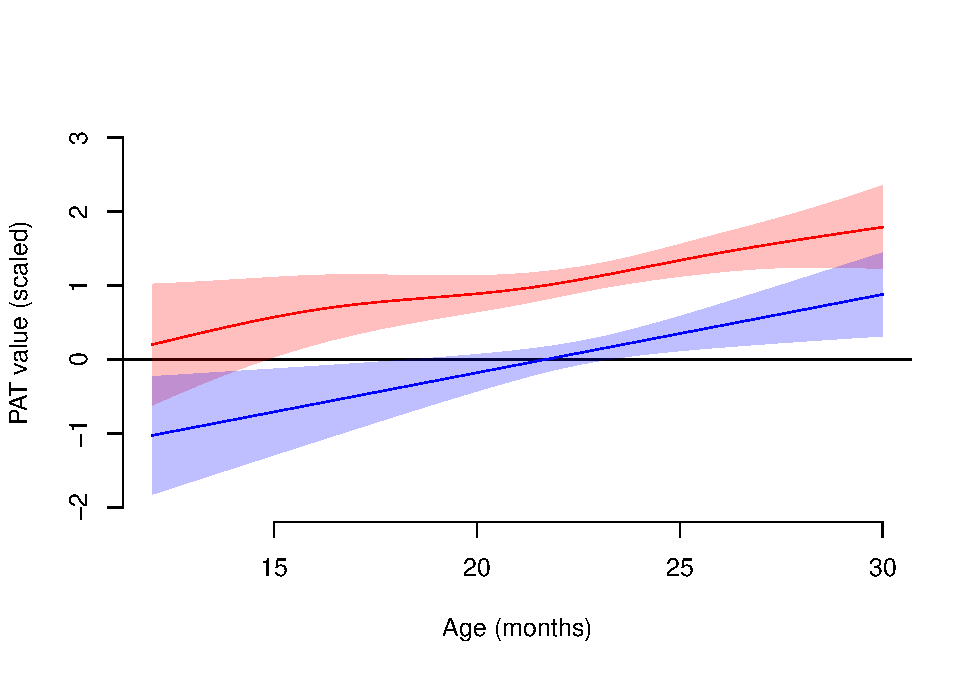
\includegraphics{PhonNetworksProj-anon_files/figure-latex/figure-GAMM-PAT-1.pdf}
\caption{\label{fig:figure-GAMM-PAT}PAT values over time in Actual and Target data, weighted according to accumulative vocabulary size. Blue line represents Actual values, red line represents Target values; coloured bands represent 95\% CIs.}
\end{figure}

\begin{figure}
\centering
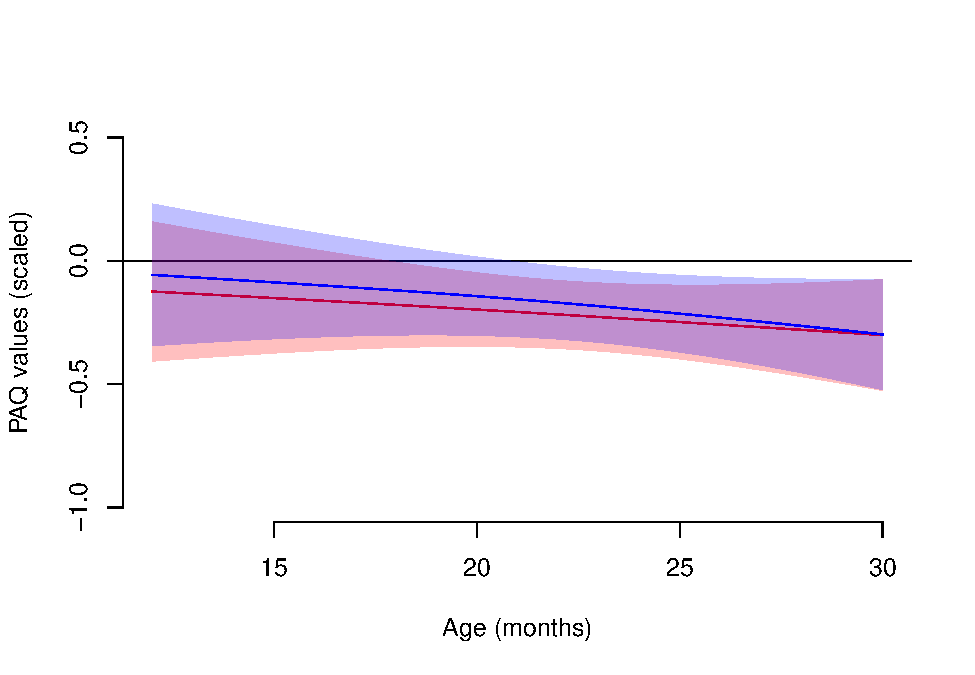
\includegraphics{PhonNetworksProj-anon_files/figure-latex/figure-GAMM-PAQ-1.pdf}
\caption{\label{fig:figure-GAMM-PAQ}PAQ values over time in Actual and Target data, weighted according to accumulative vocabulary size. Blue line represents Actual values, red line represents Target values; coloured bands represent 95\% CIs. Both smooths are shown here for exploratory purposes.}
\end{figure}

Outputs from model comparisons are shown in Table \ref{tab:table-GAMM-outputs} (rows 1-2). Consistent with the interactions reported from the logistic regression models above, age had a significant effect on PAT values in both Actual and Target data. However, the PAQ x Age interaction shown in the regression models was not supported by GAMMs. Model smooths for both PAT and PAQ are plotted in Figures \ref{fig:figure-GAMM-PAT} and \ref{fig:figure-GAMM-PAQ}; these plots show clear linear changes in PAT values over time, for both PAT and PAQ values.. In support of the findings above, and contrary to the expectations set out in H2, in the Actual data (shown in blue in Figure \ref{fig:figure-GAMM-PAT}), PAT values were lower in earlier acquisition, and increased over time. Furthermore, the trajectory is identical for the Target data (shown in red), which contrasts with the regression model outputs above. Again as suggested above, the trajectory for PAQ is negative, such that higher PAQ values occur at earlier age points.

\hypertarget{data-type-comparisons}{%
\subsubsection{Data type comparisons}\label{data-type-comparisons}}

H3 predicted that systematicity would be stronger in Actual, compared to Target, data. We would therefore expect PAT values to be higher in Actual data overall, indicating more connectivity. This analysis only applies to PAT, given that the global network used to determine PAQ-like growth is generated from Target forms anyway; the expected substantial overlap in the two data types is shown in Figure \ref{fig:figure-GAMM-PAQ}. To test for an effect of data type, GAMMs were used to account for any non-linearity in the data over time. Model structure was almost identical to that reported above, except that 1) data type was included as a parametric term, with a difference smooth\footnote{Difference smooths account for the fact that the different levels of the smooth might differ in their non-linearity; in this instance, the by-data type difference smooth accounts for the possibility that Actual and Target data may have different trajectories.} and a by-data type random smooth for the effect of age; 2) the full dataset, incorporating Actual and Target forms together, was tested.

Results from a nested model comparison are shown in Table \ref{tab:table-GAMM-outputs} (row 3). Data type had a significant effect on PAT values. A summary of the full model reveals that PAT values were significantly lower in the Target data than the Actual data (\emph{b}=-0.69, \emph{p}\textless{} .001), thereby supporting H3.

\begin{figure}
\centering
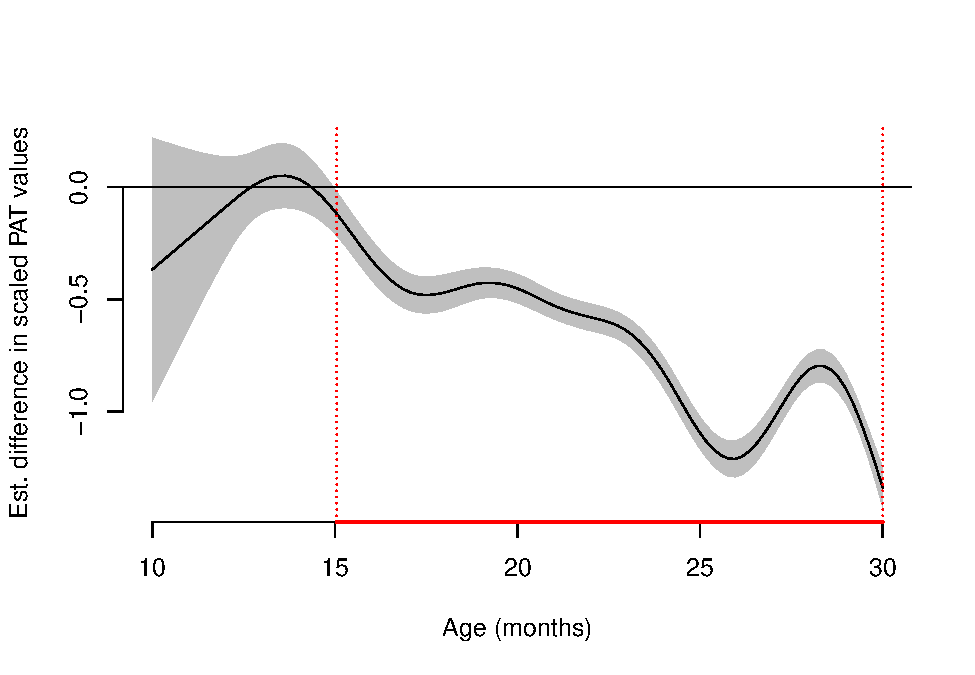
\includegraphics{PhonNetworksProj-anon_files/figure-latex/difference-smooth-data-type-1.pdf}
\caption{\label{fig:difference-smooth-data-type}Difference smooth plot showing difference between scaled PAT values in Actual vs.~Target forms from the GAMM model specified above. Shaded area shows 95\% confidence intervals, red line along x-axis indicates months in which
the difference between Actual and Target forms was significant.}
\end{figure}

The difference of the two smooths is shown in Figure \ref{fig:difference-smooth-data-type}. The red line indicates periods where the two trajectories differed significantly from one another - from 15 months until the final time-point in the analysis. For clarity, the two smooths are visualised in Figure \ref{fig:plotted-smooth-data-type} where the difference between the two trajectories is clear.

\begin{figure}
\centering
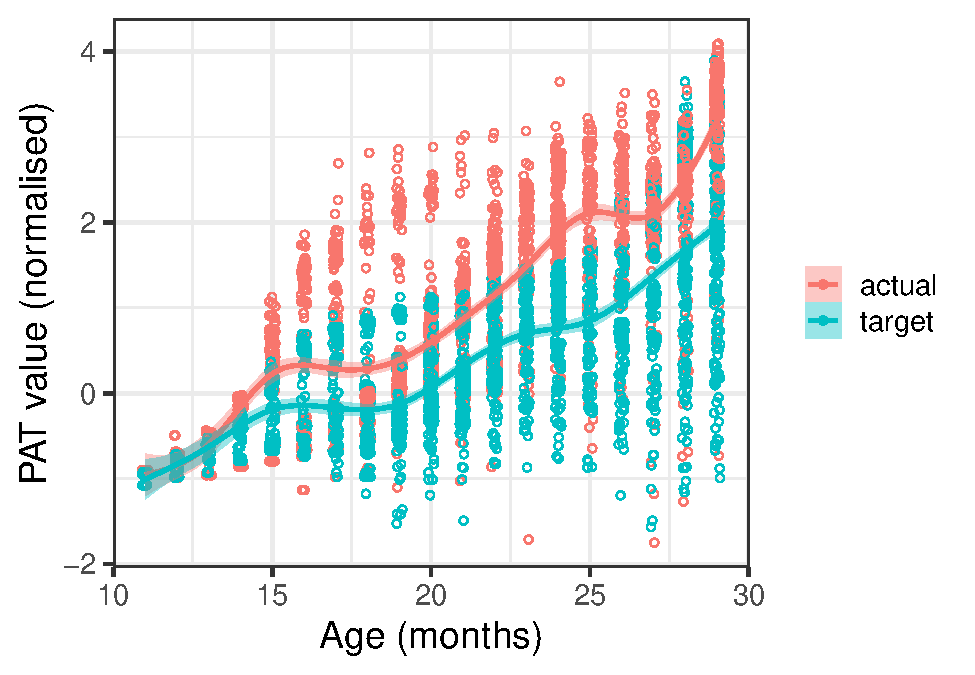
\includegraphics{PhonNetworksProj-anon_files/figure-latex/plotted-smooth-data-type-1.pdf}
\caption{\label{fig:plotted-smooth-data-type}Smooth plot showing scaled PAT values in Actual vs.~Target forms. Shaded areas show 95\% confidence intervals, lines indicate mean trajectories over time, coloured circles represent individual datapoints, jittered for visual clarity.}
\end{figure}

\hypertarget{discussion}{%
\section{Discussion}\label{discussion}}

This study tested two established frameworks of network growth in the context of early phonological development: preferential attachment (PAT) and preferential acquisition (PAQ) (Fourtassi et al., 2020; Hills et al., 2009; Siew \& Vitevitch, 2020). Using naturalistic data to quantify infants' realization of words, it was possible to establish similarity (or connectedness) across the phonological properties of infants' early words, and map how this changes over time. Based on previous analyses showing that infants' early productions tend to share phonological properties (e.g. Vihman, 2016; Waterson, 1971; see also Vihman \& Keren-Portnoy, 2013), it was hypothesised that the early vocabulary would grow in a PAT-like manner (H1) -- that is, should constitute dense clusters of similar-sounding forms -- and that acquisition should be most systematic earlier on in development (H2). Expanding on two key studies in this area (Fourtassi et al., 2020; Siew \& Vitevitch, 2020), it was also predicted that a network consisting of infants' actual productions (that is, the child's \emph{realization} of the target forms) should demonstrate more typical PAT-like growth than an equivalent network constituting just the target forms (H3). Two of these three hypotheses were supported by the data.

First, in support of H1, network growth models showed strong evidence for PAT-like growth in both Actual and Target data; newly-acquired words were produced in a similar way to existing words in the network, such that, in an given month, the most highly-connected unknown words were more likely to acquired in the next month. PAQ-like growth did not convincingly predict learning: Model 3 showed PAQ to be a significant predictor of word learning alongside PAT, but inspection of the model estimates showed that words with \emph{lower} PAQ values were more likely to be acquired, and that this effect was only marginally significant. H2 predicted that PAT-like network growth would be stronger in earlier development, based on previous analyses that show infants' earliest words to be phonologically similar or even identical (e.g. Deuchar \& Quay, 2000). However, the opposite was true: in both Actual and Target data, earlier-acquired words tended to have \emph{lower} PAT values, while later-acquired words had higher PAT values. Finally, in support of H3, PAT-like growth was more convincing for the Actual than the Target data: analysis of GAMM smooths revealed that data type (Actual versus Target) accounted for significant variance in PAT values, whereby Target data had significantly lower PAT values than Actual data from very early on in the data (15 months).

It was surprising to find so little evidence for PAQ across the analyses, given that previous studies show more convincing evidence for PAQ overall, and that PAT and PAQ are not mutually exclusive models of network growth. Amatuni and Bergelson (2017) propose that PAT and PAQ could work together, such that PAQ may ``{[}supplement{]} PAT by providing a structured sampling space for new word selection'' (p.5). That is, a combination of PAT and PAQ would provide both internal (output-driven) and external (input-driven) roles in development. Given that acquisition is a dynamic and interactive process (Thelen \& Smith, 1996), with ample evidence showing the effects of the input on early word learning (Ambridge, Kidd, Rowland, \& Theakston, 2015; Rowe, 2012), it is to be expected that both models would be at work simultaneously during acquisition. The fact that this was not shown in the current data could be due to the fact that the regression models controlled for many external factors known to affect word learning -- input frequency, word length, word category, etc. -- which together could have accounted for much of the variability that otherwise would have been captured by PAQ growth values in this corpus of naturalistic data.

The present analysis sheds new light on systematicity in early language acquisition, specifically regarding the role of PAT- and PAQ-like models of phonological development. Previous studies have drawn on age of acquisition data, using the target form as the index of production (Fourtassi et al., 2020; Siew \& Vitevitch, 2020). This has allowed study of vocabulary growth across a large sample, and findings have presented a new perspective on the role of phonological neighbourhoods in early acquisition. However, these analyses have not interrogated the role of \emph{production}. By considering networks in relation to the way infants produce their early-acquired words, it has been possible to consider phonological network growth from a novel perspective. The findings presented here reveal a systematic approach to early phonological development, as infants exploit their existing production capacity to produce new words with familiar articulatory routines. These results support many previous studies that show lexical development to take place via the implementation of systematic structures and templates (Vihman, 2019; Vihman \& Keren-Portnoy, 2013; Waterson, 1971), and also model a new way of analysing phonological systematicity in infants' early productions, which can be extended to larger samples and applied to a wider variety of languages.

Given that Fourtassi and colleagues (2020) analysed data from children of similar ages using the same subset of words (i.e.~CDI words), we would expect the current findings to map on to their results, particularly in the analysis of Target data. And indeed, this is the area where we find the most evidence for PAQ-like network growth. However, their study reveals consistently stronger evidence for PAQ and so our results do not align as much as might be expected. This may reflect direct differences in the type of data used: in the present study, the order of acquisition (and thereby the model of network growth) reflects the chronological order of individual children's production. Month-by-month acquisition norms taken from thousands of children's CDIs model an `average' order of acquisition, whereby words that \emph{tend to} appear earlier in the developing lexicon are biased towards an earlier age of acquisition. Frank and colleagues (2021) report the first 10 words of infants acquiring American English, which (for stop consonants only) contain two instances of /m/, three each of /n/ and /d/, five /b/ and one /g/. In naturalistic production, however, a word's phonological form may prime the acquisition of other similar-sounding words: production of \emph{baby} may be shortly followed by \emph{bib} and \emph{ball} (cf. McCune \& Vihman, 2001), while in vocabulary norms, acquisition of \emph{baby}, \emph{bib} and \emph{ball} is represented at the group level. Vocabulary norming data thus represents an `averaging out' of phonological connectedness across thousands of infants, creating a bias towards PAQ-like growth. Previous similar studies perhaps represent a more general, one-size-fits-all trajectory to lexical development, whereas these results capture individual clusters of connectivity as children acquire words that match the phonological characteristics of existing words in the lexicon.

Indeed, studies of infants' early words show that, on a word-by-word basis, early-acquired forms tend to consist of the same set of consonants, in both target and actual forms. This reflects the child's `selection' of early words to match their own consonant repertoire (McCune \& Vihman, 2001; Stoel-Gammon \& Cooper, 1984; Vihman, 2019). Given that these results show evidence for PAT-like growth in both Actual and Target data, it appears that infants are selectively acquiring forms that match their own production preferences, and are either producing these forms accurately (\emph{selected}, in Vihman's terms) or \emph{adapting} them to match their preferred output patterns. Within Vihman's framework, phonological development involves the selection or adaption of lexical units to fit a set of easily-accessible articulatory categories. That is, an infant systematically acts upon new understanding (i.e.~acquired receptive vocabulary items) within the limitations of their development, selecting existing categories to deal with challenges presented in production. These are `well-worn paths' that represent the stable and well-rehearsed production routines that drive selection, and later adaption, of infants' early word forms. In producing forms that are accessible and familiar to the child, they can `rehearse' particular segments and structures, easing up memory and planning capacity for more flexible and variable production further down the line.

This study raises new questions for future analyses into systematicity in phonological development. While efforts were made to fully characterise the phonological content of infants' early productions -- through using distinctive features with Euclidean, rather than Levenshtein, distance, and observing Actual productions alongside Target forms -- still it was not possible to capture the full extent of systematicity, i.e.~the presence of prosodic structures or templates (Vihman, 2019). Future work in this area should expand the analyses to consider the development and systematic implementation of templates. Furthermore, this analysis considers only two languages; it would be valuable to extend the approach to a wider variety of languages. Indeed, systematicity has been demonstrated across languages (Arnon \& Clark, 2011; Khattab \& Al-Tamimi, 2013; Szreder, 2013), and so it should be possible to find cross-linguistic commonalities in network growth. Typological differences in network growth would raise questions about the cognitive reality of systematicity in phonological development.

\hypertarget{conclusion}{%
\section{Conclusion}\label{conclusion}}

When naturalistic data is considered within a networks account, we find evidence for PAT-like network growth, but not PAQ-like growth. English- and French-learning infants acquired words that would connect to the most highly-connected nodes in the existing network (PAT-like growth), and this became increasingly systematic over time. When we look at the target form of the words infants acquire and how they produce them, in both cases we see evidence to show that early acquisition is driven -- at least in part -- by preferences in the output. That is, infants acquire words that cluster together phonologically, and produce them systematically such that early production represents clusters of similar-sounding forms.

\newpage

\hypertarget{references}{%
\section{References}\label{references}}

\begingroup
\setlength{\parindent}{-0.5in}
\setlength{\leftskip}{0.5in}

\hypertarget{refs}{}
\begin{CSLReferences}{1}{0}
\leavevmode\vadjust pre{\hypertarget{ref-amatuni_semantic_2017}{}}%
Amatuni, A., \& Bergelson, E. (2017). \emph{Semantic networks generated from early linguistic input} {[}Preprint{]}. Animal Behavior; Cognition. \url{https://doi.org/10.1101/157701}

\leavevmode\vadjust pre{\hypertarget{ref-ambridge_ubiquity_2015}{}}%
Ambridge, B., Kidd, E., Rowland, C. F., \& Theakston, A. L. (2015). The ubiquity of frequency effects in first language acquisition. \emph{Journal of Child Language}, \emph{42}(2), 239--273. \url{https://doi.org/10.1017/S030500091400049X}

\leavevmode\vadjust pre{\hypertarget{ref-arnon_experience_2011}{}}%
Arnon, I., \& Clark, E. V. (2011). \emph{Experience, variation and generalization: Learning a first language}. John Benjamins Publishing.

\leavevmode\vadjust pre{\hypertarget{ref-R-lme4}{}}%
Bates, D., Mächler, M., Bolker, B., \& Walker, S. (2015). Fitting linear mixed-effects models using {lme4}. \emph{Journal of Statistical Software}, \emph{67}(1), 1--48. \url{https://doi.org/10.18637/jss.v067.i01}

\leavevmode\vadjust pre{\hypertarget{ref-bell_network_2017}{}}%
Bell, M., Perera, S., Piraveenan, M., Bliemer, M., Latty, T., \& Reid, C. (2017). Network growth models: A behavioural basis for attachment proportional to fitness. \emph{Scientific Reports}, \emph{7}(1), 42431. \url{https://doi.org/10.1038/srep42431}

\leavevmode\vadjust pre{\hypertarget{ref-chomsky_noam_sound_1968}{}}%
Chomsky, Noam, \& Halle, Morris. (1968). \emph{The sound pattern of english}. New York, {NY}: Harper; Rowe.

\leavevmode\vadjust pre{\hypertarget{ref-demuth_katherine_prosodically-conditioned_2008}{}}%
Demuth, Katherine, \& Tremblay, Annie. (2008). Prosodically-conditioned variability in children's production of french determiners. \emph{Journal of Child Language}, \emph{35}(1). Retrieved from \url{https://www-cambridge-org.abc.cardiff.ac.uk/core/journals/journal-of-child-language/article/prosodicallyconditioned-variability-in-childrens-production-of-french-determiners/B34D994A1EA63DFF841D1C2C7974D6FE}

\leavevmode\vadjust pre{\hypertarget{ref-demuth_word-minimality_2006}{}}%
Demuth, K., Culbertson, J., \& Alter, J. (2006). Word-minimality, epenthesis and coda licensing in the early acquisition of english. \emph{Language and Speech}, \emph{49}(2), 137--174.

\leavevmode\vadjust pre{\hypertarget{ref-deuchar_bilingual_2000}{}}%
Deuchar, M., \& Quay, S. (2000). \emph{Bilingual acquisition: Theoretical implications of a case study}. Oxford, {UK}: Oxford University Press.

\leavevmode\vadjust pre{\hypertarget{ref-donegan_normal_2013}{}}%
Donegan, P. (2013). Normal vowel development. In M. J. Ball \& F. E. Gibbons (Eds.), \emph{Handbook of vowels and vowel disorders} (pp. 24--60). Psychology Press.

\leavevmode\vadjust pre{\hypertarget{ref-fenson_variability_1994}{}}%
Fenson, L., Dale, P. S., Reznick, J. S., Bates, E., Thal, D. J., Pethick, M., Stephen J. Tomasello, \ldots{} Stiles, J. (1994). Variability in early communicative development. \emph{Monographs of the Society for Research in Child Development}, \emph{59}. \url{https://doi.org/10.2307/1166093}

\leavevmode\vadjust pre{\hypertarget{ref-ferguson_words_1975}{}}%
Ferguson, Charles. A., \& Farwell, C. B. (1975). Words \& sounds in early language acquisition. \emph{Language}, \emph{51}, 419--439.

\leavevmode\vadjust pre{\hypertarget{ref-fourtassi_growth_2020}{}}%
Fourtassi, A., Bian, Y., \& Frank, M. C. (2020). The growth of children's semantic and phonological networks: Insight from 10 languages. \emph{Cognitive Science}, \emph{44}(7), e12847. \url{https://doi.org/10.1111/cogs.12847}

\leavevmode\vadjust pre{\hypertarget{ref-frank_wordbank_2017}{}}%
Frank, M. C., Braginsky, M., Yurovsky, D., \& Marchman, V. A. (2017). Wordbank: An open repository for developmental vocabulary data. \emph{Journal of Child Language}, \emph{44}(3), 677--694. \url{https://doi.org/10.1017/S0305000916000209}

\leavevmode\vadjust pre{\hypertarget{ref-frank_variability_2021}{}}%
Frank, M. C., Braginsky, M., Yurovsky, D., \& Marchman, V. A. (2021). \emph{Variability and consistency in early language learning: The wordbank project}. {MIT} Press.

\leavevmode\vadjust pre{\hypertarget{ref-hedlund_gregory_phon_2020}{}}%
Hedlund, G., \& Rose, Y. (2020). \emph{Phon 3.1 {[}computer software{]}}. Retrieved from \url{https://phon.ca}

\leavevmode\vadjust pre{\hypertarget{ref-hills_longitudinal_2009}{}}%
Hills, T. T., Maouene, M., Maouene, J., Sheya, A., \& Smith, L. (2009). Longitudinal analysis of early semantic networks preferential attachment or preferential acquisition? \emph{Psychological Science}, \emph{20}(6), 729--739. \url{https://doi.org/10.1111/j.1467-9280.2009.02365.x}

\leavevmode\vadjust pre{\hypertarget{ref-jones_children_2019}{}}%
Jones, S., \& Brandt, S. (2019). Do children really acquire dense neighbourhoods? \emph{Journal of Child Language}, \emph{46}(6), 1260--1273. \url{https://doi.org/10.1017/S0305000919000473}

\leavevmode\vadjust pre{\hypertarget{ref-kent_what_2020}{}}%
Kent, R. D., \& Rountrey, C. (2020). What acoustic studies tell us about vowels in developing and disordered speech. \emph{American Journal of Speech-Language Pathology}, \emph{29}(3), 1749--1778. \url{https://doi.org/10.1044/2020_AJSLP-19-00178}

\leavevmode\vadjust pre{\hypertarget{ref-kern_sophie_ifdc_2010}{}}%
Kern, S., \& Gayraud, F. (2010). \emph{{IFDC}}. Grenoble: Les éditions la cigale.

\leavevmode\vadjust pre{\hypertarget{ref-khattab_influence_2013}{}}%
Khattab, G., \& Al-Tamimi, J. (2013). Influence of geminate structure on early arabic templatic patterns. In M. M. Vihman \& T. Keren-Portnoy (Eds.), \emph{The emergence of phonology: Whole-word approaches and cross-linguistic evidence} (pp. 374--414). Cambridge: Cambridge University Press. \url{https://doi.org/10.1017/CBO9780511980503.018}

\leavevmode\vadjust pre{\hypertarget{ref-macwhinney_childes_2000}{}}%
MacWhinney, B. (2000). \emph{The {CHILDES} project: Tools for analyzing talk} (3rd ed.). Mahwah, {NJ}: Lawrence Erlbaum Associates. \url{https://doi.org/10.1177/026565909200800211}

\leavevmode\vadjust pre{\hypertarget{ref-mak_evidence_2020}{}}%
Mak, M. H. C., \& Twitchell, H. (2020). Evidence for preferential attachment: Words that are more well connected in semantic networks are better at acquiring new links in paired-associate learning. \emph{Psychonomic Bulletin \& Review}, \emph{27}(5), 1059--1069. \url{https://doi.org/10.3758/s13423-020-01773-0}

\leavevmode\vadjust pre{\hypertarget{ref-mccune_early_2001}{}}%
McCune, L., \& Vihman, M. M. (2001). Early phonetic and lexical development. \emph{Journal of Speech, Language, and Hearing Research}, \emph{44}(3), 670--684. \url{https://doi.org/10.1044/1092-4388(2001/054)}

\leavevmode\vadjust pre{\hypertarget{ref-mcleod_childrens_2018}{}}%
McLeod, S., \& Crowe, K. (2018). Children's consonant acquisition in 27 languages: A cross-linguistic review. \emph{American Journal of Speech-Language Pathology}, \emph{27}(4), 1546--1571. \url{https://doi.org/10.1044/2018_AJSLP-17-0100}

\leavevmode\vadjust pre{\hypertarget{ref-mitchell_cognates_2022}{}}%
Mitchell, L., Tsui, R. K. Y., \& Byers-Heinlein, K. (2022). \emph{Cognates are advantaged in early bilingual expressive vocabulary development}. {PsyArXiv}. \url{https://doi.org/10.31234/osf.io/daktp}

\leavevmode\vadjust pre{\hypertarget{ref-monaghan_measures_2010}{}}%
Monaghan, P., Christiansen, M. H., Farmer, T. A., \& Fitneva, S. A. (2010). Measures of phonological typicality. \emph{The Mental Lexicon}, \emph{5}(3), 281--299. \url{https://doi.org/10.1075/ml.5.3.02mon}

\leavevmode\vadjust pre{\hypertarget{ref-R-base}{}}%
R Core Team. (2020). \emph{R: A language and environment for statistical computing}. Vienna, Austria: R Foundation for Statistical Computing. Retrieved from \url{https://www.R-project.org/}

\leavevmode\vadjust pre{\hypertarget{ref-R-itsadug}{}}%
Rij, J. van, Wieling, M., Baayen, R. H., \& Rijn, H. van. (2022). \emph{{itsadug}: Interpreting time series and autocorrelated data using GAMMs}.

\leavevmode\vadjust pre{\hypertarget{ref-rowe_longitudinal_2012}{}}%
Rowe, M. L. (2012). A longitudinal investigation of the role of quantity and quality of child-directed speech in vocabulary development. \emph{Child Development}, \emph{83}(5), 1762--1774. \url{https://doi.org/10.1111/j.1467-8624.2012.01805.x}

\leavevmode\vadjust pre{\hypertarget{ref-seidenberg_dyslexia_1999}{}}%
Seidenberg, M. S., Harm, M. W., \& Seidenberg, M. S. (1999). Dyslexia: Insights from connectionist models. \emph{Unpublished Doctoral Dissertation, University of Southern California, Los}, 491--528.

\leavevmode\vadjust pre{\hypertarget{ref-siew_investigation_2020}{}}%
Siew, C. S. Q., \& Vitevitch, M. S. (2020). An investigation of network growth principles in the phonological language network. \emph{Journal of Experimental Psychology: General}. \url{https://doi.org/10.1037/xge0000876}

\leavevmode\vadjust pre{\hypertarget{ref-soskuthy_generalised_2017}{}}%
Sóskuthy, M. (2017). \emph{Generalised additive mixed models for dynamic analysis in linguistics: A practical introduction}. arXiv. Retrieved from \url{http://arxiv.org/abs/1703.05339}

\leavevmode\vadjust pre{\hypertarget{ref-steyvers_large-scale_2005-2}{}}%
Steyvers, M., \& Tenenbaum, J. B. (2005). The large-scale structure of semantic networks: Statistical analyses and a model of semantic growth. \emph{Cognitive Science}, \emph{29}(1), 41--78. \url{https://doi.org/10.1207/s15516709cog2901_3}

\leavevmode\vadjust pre{\hypertarget{ref-stoel-gammon_patterns_1984}{}}%
Stoel-Gammon, C., \& Cooper, J. A. (1984). Patterns of early lexical and phonological development. \emph{Journal of Child Language}, \emph{11}(2), 247--271. \url{https://doi.org/10.1017/S0305000900005766}

\leavevmode\vadjust pre{\hypertarget{ref-szreder_acquisition_2013}{}}%
Szreder, M. (2013). The acquisition of consonant clusters in polish: A case study. In M. M. Vihman \& T. Keren-Portnoy (Eds.), \emph{The emergence of phonology: Whole-word approaches and cross-linguistic evidence} (pp. 343--361). Cambridge: Cambridge University Press. \url{https://doi.org/10.1017/CBO9780511980503.016}

\leavevmode\vadjust pre{\hypertarget{ref-thelen_esther_dynamic_1996}{}}%
Thelen, E., \& Smith, L. (1996). \emph{A dynamic systems approach to the development of cognition and action.} Boston, {MA}: {MIT} Press.

\leavevmode\vadjust pre{\hypertarget{ref-vihman_phonological_2014}{}}%
Vihman, M. M. (2014). \emph{Phonological development: The first two years} (2nd ed.). Malden, {MA}: Wiley-Blackwell.

\leavevmode\vadjust pre{\hypertarget{ref-vihman_prosodic_2016}{}}%
Vihman, M. M. (2016). Prosodic structures and templates in bilingual phonological development. \emph{Bilingualism: Language and Cognition}, \emph{19}(1), 69--88. \url{https://doi.org/10.1017/S1366728914000790}

\leavevmode\vadjust pre{\hypertarget{ref-vihman_phonological_2019}{}}%
Vihman, M. M. (2019). \emph{Phonological templates in development}. Oxford, {UK}: Oxford University Press.

\leavevmode\vadjust pre{\hypertarget{ref-vihman_external_1994}{}}%
Vihman, M. M., Kay, E., Boysson-Bardies, B. de, Durand, C., \& Sundberg, U. (1994). External sources of individual differences? A cross-linguistic analysis of the phonetics of mothers' speech to 1-year-old children. \emph{Developmental Psychology}, \emph{30}(5), 651--662.

\leavevmode\vadjust pre{\hypertarget{ref-vihman_emergence_2013}{}}%
Vihman, M. M., \& Keren-Portnoy, T. (2013). The emergence of phonology: Whole-word approaches, cross-linguistic evidence. In M. M. Vihman \& T. Keren-Portnoy (Eds.), \emph{The emergence of phonology: Whole-word approaches and cross-linguistic evidence}. Cambridge: Cambridge University Press. \url{https://doi.org/10.1017/CBO9780511980503.002}

\leavevmode\vadjust pre{\hypertarget{ref-waterson_child_1971}{}}%
Waterson, N. (1971). Child phonology : A prosodic view. \emph{Journal of Linguistics}, \emph{7}(2), 179--211. \url{https://doi.org/10.1017/S0022226700002917}

\leavevmode\vadjust pre{\hypertarget{ref-wieling_analyzing_2018}{}}%
Wieling, M. (2018). Analyzing dynamic phonetic data using generalized additive mixed modeling: {A} tutorial focusing on articulatory differences between {L1} and {L2} speakers of {English}. \emph{Journal of Phonetics}, \emph{70}, 86--116. \url{https://doi.org/10.1016/j.wocn.2018.03.002}

\leavevmode\vadjust pre{\hypertarget{ref-R-mgcv_a}{}}%
Wood, S. N. (2011). Fast stable restricted maximum likelihood and marginal likelihood estimation of semiparametric generalized linear models. \emph{Journal of the Royal Statistical Society (B)}, \emph{73}(1), 3--36.

\end{CSLReferences}

\textbackslash end\{longtable\}
\endgroup


\end{document}
